\documentclass[12pt]{article}

\usepackage{sbc-template}
\usepackage{graphicx,url}
\def\UrlBreaks{\do\/}
\usepackage[utf8]{inputenc}
\usepackage[brazil]{babel}

\sloppy

\title{GPV: Sistema de gerenciamento de viagens}

\author{Cristian Edson Meneghetti, {\small Diego Antonio Lusa (Orientador)}}


\address{Instituto Federal de Ciência e Tecnologia do Rio Grande do Sul IFRS - Campus Sertão\\
  Caixa Postal 21 -- 99.170-000 -- Sertão -- RS -- Brazil
  \email{cristianedsonm@gmail.com, diego.lusa@sertao.ifrs.edu.br}
}

\begin{document} 

\maketitle

\begin{abstract}
  This meta-paper describes the style to be used in articles and short papers
  for SBC conferences. For papers in English, you should add just an abstract
  while for the papers in Portuguese, we also ask for an abstract in
  Portuguese (``resumo''). In both cases, abstracts should not have more than
  10 lines and must be in the first page of the paper.
\end{abstract}
     
\begin{resumo} 
Manchete. elementos necessários: instituto, curso, tcc, objetivo, resultado 10 linhas. Este meta-artigo descreve o estilo a ser usado na confecção de artigos e  resumos de artigos para publicação nos anais das conferências organizadas  pela SBC. É solicitada a escrita de resumo e abstract apenas para os artigos  escritos em português. Artigos em inglês deverão apresentar apenas abstract.  Nos dois casos, o autor deve tomar cuidado para que o resumo (e o abstract)  não ultrapassem 10 linhas cada, sendo que ambos devem estar na primeira página do artigo.
\end{resumo}


\section{Introdução}

Resumo expandido. Com seu ultimo paragrafo ele deverá dizer a estrutura do artigo, como um micro sumário descritivo todos os tópicos após os objetivos são fundamentados em referências de autores relevante, frameworks e outros itens não vistos no curso podem ser explicados de forma mais profunda.

\section{Definição do problema e justificativa} \label{sec:firstpage}

O gerenciamento de viagens de passageiros fretadas apresenta um desafio para as empresas que as ofertam. Especialmente as que ofertam múltiplos serviços, com funcionamento paralelo, enfrentam isso gera o desafio de controlar o número de passageiros para um destino em dias e turnos distintos e quais veículos e motoristas estariam disponíveis nesses períodos. Essas informações são vitais para identificar modos de utilizar a frota da empresa de forma mais eficiente.

A utilização de softwares gerenciais pode ser de grande ajuda para empresas de transporte e turismo. Segundo \cite{perp}, a utilização de um sistema para auxiliar as escalas de trabalho de motoristas, proporcionou a redução dos custos com horas extras, além de monitorar outros custos de operação. No entanto, algumas empresas que trabalham com fretamento de sua frota, acabam por oferecer planos de viagens que se assemelham a assinaturas em conjunto com venda de passagens, com ou sem reserva de poltrona, sendo que por vezes, mais de um serviço é ofertado simultaneamente.

Adicionalmente, existem normas e regulamentos que regem o transporte de passageiros. A ANTT (Agência Nacional de Transporte Terrestres) é uma agência brasileira responsável pela regulamentação do transporte de passageiros e cargas, em rodovias e ferrovias. Duas normas publicadas pela ANTT justificam a existência de um controle apurado das operações das empresas, essas são as resoluções 4770/2015 \cite{br:2015} que exige o cadastramento da frota e a resolução 1971/2007 \cite{br:2007} que exige o cadastramento de motoristas. Sendo assim, o controle das operações realizadas por uma empresa são uma necessidade gerencial e legal, definida pela legislação brasileira e, consequentemente, se não for cumprida resultará em consequências judiciais.

Assim, evidencia-se a necessidade de utilizar um método eficiente de organizar os planos de viagem e outros aspectos da operação de uma empresa do ramo de transporte de passageiros. Para suprir essa necessidade do mercado, algumas empresas desenvolveram ERPs, como, por exemplo, a \cite{praxio}, que desenvolveu o Praxio Globus. Outra empresa é a \cite{easy} que criou o Easytrans. Ambos os softwares procuram possibilitar para a empresa um modelo de gestão completa das operações internas, mediante um contrato firmado entre a empresa utilizadora do sistema e sua desenvolvedora. No caso da Praxio Globus, é ofertada uma apresentação do software mediante agendamento. Também existem algumas empresas que ofertam a compra de passagens de ônibus, como a \cite{busbud} que desenvolve o serviço Busbud tanto no formato web como aplicativo para dispositivos móveis, também a \cite{qp} que criou o site Quero Passagem. No entanto, estes são focados unicamente em empresas que trabalham com a venda tradicional de passagens, com reserva de poltrona.

Com base no que foi levantando, de acordo com informações disponibilizadas pela \cite{easy} seu produto o Easytrans é baseado em tecnologias legadas, porém ainda assim possui as funções necessárias para a gestão eficiente do negócio. O Easytrans por sua vez é desenvolvido exclusivamente para desktop com o framework Delphi para a plataforma Windows, limitando o número de plataformas suportadas pelo mesmo. Já o Praxio Globus opera em formato web com a utilização de modularização, proporcionando diferentes módulos de gestão que se adéquam as necessidades do cliente. Recentemente, passou a ser ofertado como um módulo do software Praxio Globus a venda de passagens com reserva de poltrona ao embarcar, sem necessidade de quiosques de venda. Quanto aos sites de venda de passagens disponíveis ao público em geral, o Busbud está disponível em diversos países da América do Norte, Sul e Europa segundo informações de seu desenvolvedor a \cite{busbud} e o Quero Passagem possui abrangência limitada ao mercado brasileiro de transporte de passageiros.

Os softwares citados cumprem sua função, e com exceção do Easytrans estão disponíveis para usuários de um grande número de plataformas, no entanto, eles não cobrem a operação de todas as empresas de transporte de passageiros. Um exemplo, são as que operam de forma mista, ou seja, ofertando passagem e assinatura de serviço ou não operam com reserva de poltrona. Por não contemplarem em seu desenvolvimento estes serviços diferenciados, estes sistemas não possuem a possibilidade de interação entre os passageiros e a empresa em um formato adequando, principalmente para as empresas que ofertam a assinatura mensal dos seus serviços, para um determinado destino. 

Portanto, embora haja a oferta de softwares competentes, que seguem a legislação brasileira para as empresas de transporte de passageiros, e estes auxiliem os processos operacionais e gerenciais, não foram encontrados sistemas que atendem operações mistas ou em regime que se assemelhe a uma assinatura. Consequentemente, empresas que ofertam serviços nesse modelo, poderiam se beneficiar de controles projetados para suas necessidades, e também, aumentar a eficiência e eficácia do seu controle de passageiros, seja pela criação de um canal direto de comunicação entre os usuários e a empresa contratada, seja pelo auxílio a cumprir as normas nacionais para a operação da empresa em território brasileiro.

\section{Objetivos}
Em relação aos elementos elencados para o sistema foram definidos em dois itens objetivo geral e objetivos específicos.
\subsection{Objetivo Geral}
 Prover um software para gerir, de forma eficientes, as operações diárias de empresas de transporte de passageiros e, também, auxiliar os passageiros a comunicar suas presenças ou ausências em um determinado período, de uma rota de transporte para um destino.
\subsection{Objetivos Específicos} \begin{itemize}
	\item Disponibilizar diferentes perfis de usuários
	\item Proporcionar a autenticação de diferentes perfis de usuário.
	\item Possibilitar a gerência dos planos de viagens.
	\item Facilitar o controle de paradas dos planos.
	\item Oferecer a previsão do valor do plano de acordo com as opções escolhidas pelo cliente.
	\item Possibilitar a gerência dos usuários de um plano.
	\item Possibilitar a gerência da alocação de veículos utilizados nas viagens.
	\item Oferecer a geração de um relatório de passageiros.
	\item Possibilitar a gerência da alocação de motoristas das viagens.
	\item Facilitar o controle de presenças e ausências de passageiros em viagens.
\end{itemize}

\section{Fundamentação Teórica e Trabalhos Relacionados}

Section titles must be in boldface, 13pt, flush left. There should be an extra
12 pt of space before each title. Section numbering is optional. The first
paragraph of each section should not be indented, while the first lines of
subsequent paragraphs should be indented by 1.27 cm.

\section{Metodologia}

\subsection{Descrição do Software}
O sistema proposto visa gerenciar os destinos e planos ofertados por uma empresa do ramo de transporte de passageiros, além de seus passageiros e veículos. Ao mesmo tempo visa ajudar os clientes a reservarem o uso dos serviços de transporte ofertados pela empresa. Consequentemente, haverá a divisão do sistema em dois segmentos alvos distintos: o administrador, que mediante autenticação poderá gerenciar planos de viagem, uso de veículos, alocação de motoristas, listagem de usuários utilizadores de um plano e usuários previstos para dias e turnos específicos de um plano; e os clientes da empresa que poderão reservar vagas com a especificação de quais serão os dias e turnos que utilizarão o transporte, sendo esta reserva no regime passagem ou assinatura. Também haverá a autenticação das credencias dos usuários para o acesso ao sistema e, adicionalmente, se o usuário utilizar um plano em regime de assinatura, poderá indicar se utilizará ou não o serviço num dia especifico.

A reserva, por sua vez, passa por um controle do número de passageiros. Isso é necessário pois, um destino pode comportar tanto opções mensais como eventuais passagens. Para suprir a necessidade identificada, o sistema deve controlar o número total de passageiros, separando as viagens de ida e volta de destinos, como entidades distintas e impedir que exista um número excessivo de pessoas nessas viagens. Para haver um melhor controle de presenças, os administradores do sistema poderão visualizar, por meio de listagem, os usuários que utilizarão o serviço em um determinado turno de um dia. 

Devido à necessidade de alocar os veículos eficientemente, também será ofertado a alocação dos mesmos num plano e em qual dia da semana e turno serão utilizados, com a indicação do motorista responsável pela operação do veículo na ocasião.
O sistema não receberá os pagamentos dos usuários, assim como não possuirá o uso de catraca para a contabilização no veículo de transporte, de passageiros que utilizarem o serviço.

\subsection{Requisitos}
Requisitos segundo \cite{sommervile:2016} são os descritores de o que o sistema deve prover, as restrições impostas em sua operação e refletem as necessidades do cliente. Para documentar esse aspecto fundamental do desenvolvimento de software convém dividir estes conforme delineado por \cite{sommervile:2016} em requisitos funcionais e não funcionais. 
\subsubsection{Não Funcionais}
Como requisitos não funcionais que de acordo com \cite{sommervile:2016} são restrições nas funções ou serviços ofertados pelo sistema e muitas vezes se aplicam ao software como um todo. Os seguintes requisitos foram elencados:
\begin{itemize}
	\item Front-end: para seu desenvolvimento foi vislumbrado a criação de uma SPA (Single page application) responsável pelo acesso administrativo que permite o controle gerencial da empresa. Paralelamente um aplicativo móvel híbrido será utilizado com o uso de NativeScript para os passageiros. Em ambos os casos estes serão construídos com o conjunto de linguagens HTML, CSS e Javascript utilizando-se do framework Vue.js.
	\item Back-end: será desenvolvido com a utilização do framework Javalin que tem seu enfoque na construção de APIs REST e microsserviços. No que se refere a linguagem o Kotlin será utilizado com sua opção de compilá-lo para bytecode java para utilização em JVM.
	\item Armazenamento de dados: devido algumas características dos dados armazenados o banco orientado a grafos ArangoDB será utilizado na API e no aplicativo móvel haverá a utilização de SQLite se assim for visto a necessidade da criação de uma espécie de cache para a aplicação.
	\item Projeto: para a confecção do projeto e consequentemente a criação dos diagramas necessários para a modelagem do banco de dados serão utilizadas as ferramentas BrModelo, Dia e Astah Community. No desenvolvimento do código fonte será utilizada a IDE Intellij IDEA.
\end{itemize}

\section{Considerações Finais e Trabalhos Futuros}

Section titles must be in boldface, 13pt, flush left. There should be an extra
12 pt of space before each title. Section numbering is optional. The first
paragraph of each section should not be indented, while the first lines of
subsequent paragraphs should be indented by 1.27 cm.

\subsection{Subsections}

The subsection titles must be in boldface, 12pt, flush left.

\section{Figures and Captions}\label{sec:figs}


Figure and table captions should be centered if less than one line
(Figure~\ref{fig:exampleFig1}), otherwise justified and indented by 0.8cm on
both margins, as shown in Figure~\ref{fig:exampleFig2}. The caption font must
be Helvetica, 10 point, boldface, with 6 points of space before and after each
caption.

\begin{figure}[ht]
\centering
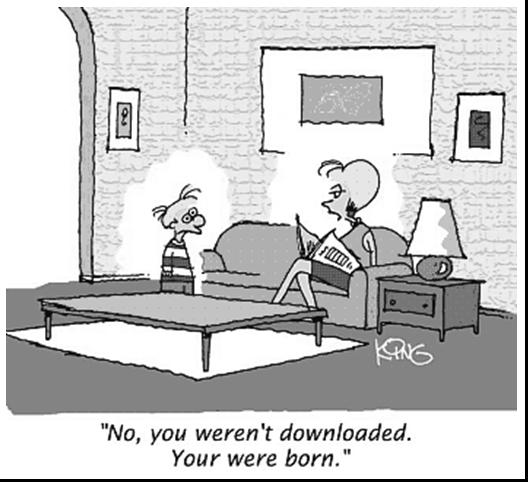
\includegraphics[width=.5\textwidth]{fig1.jpg}
\caption{A typical figure}
\label{fig:exampleFig1}
\end{figure}

\begin{figure}[ht]
\centering
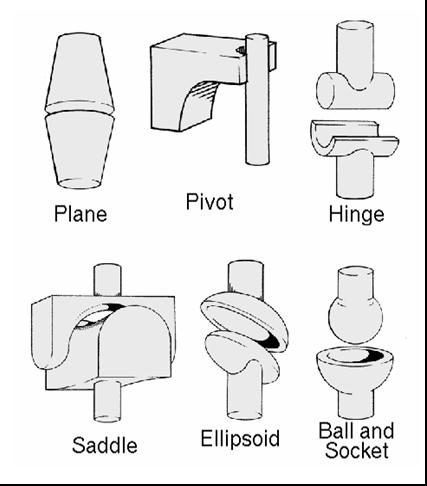
\includegraphics[width=.3\textwidth]{fig2.jpg}
\caption{This figure is an example of a figure caption taking more than one
  line and justified considering margins mentioned in Section~\ref{sec:figs}.}
\label{fig:exampleFig2}
\end{figure}

In tables, try to avoid the use of colored or shaded backgrounds, and avoid
thick, doubled, or unnecessary framing lines. When reporting empirical data,
do not use more decimal digits than warranted by their precision and
reproducibility. Table caption must be placed before the table (see Table 1)
and the font used must also be Helvetica, 10 point, boldface, with 6 points of
space before and after each caption.

\begin{table}[ht]
\centering
\caption{Variables to be considered on the evaluation of interaction
  techniques}
\label{tab:exTable1}
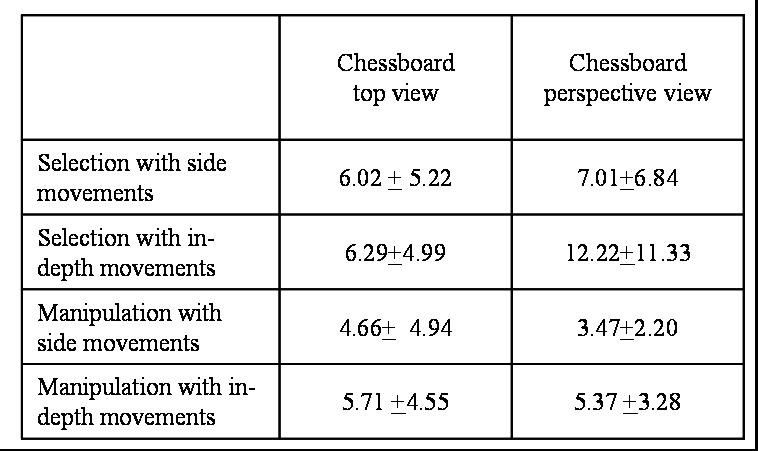
\includegraphics[width=.7\textwidth]{table.jpg}
\end{table}

\section{Images}

All images and illustrations should be in black-and-white, or gray tones,
excepting for the papers that will be electronically available (on CD-ROMs,
internet, etc.). The image resolution on paper should be about 600 dpi for
black-and-white images, and 150-300 dpi for grayscale images.  Do not include
images with excessive resolution, as they may take hours to print, without any
visible difference in the result. 

\section{References}

Bibliographic references must be unambiguous and uniform.  We recommend giving
the author names references in brackets, e.g. \cite{knuth:84},
\cite{boulic:91}, and \cite{smith:99}.

The references must be listed using 12 point font size, with 6 points of space
before each reference. The first line of each reference should not be
indented, while the subsequent should be indented by 0.5 cm.

\bibliographystyle{sbc}
\bibliography{sbc-template}

\end{document}
